\section{The SAGA Runtime System} \textbf{O.W / H.K.}

 \subsection{Design Philosophy}
 \textbf{H.K.}
 \jhanote{Why Boost?}

 \subsection{Core Components}
 
 \subsubsection{Library Design}
 
 PIMPL, etc. \textbf{H.K.}
 How it is Split up
 Late Binding
 

 \subsubsection{Runtime System}
 Adaptor selection, logging, etc. Mechanisms  \textbf{H.K.}

 
\subsection{Middleware Adaptors}
% Design, CPI, Extensibility etc... \textbf{O.W}

 One of the most important design porperties in SAGA is its vertical
 extensibility at the so-called CPI (Capability Provider Interface)
 level.  The CPI defines the boundary between the end-user \jhanote{at
   some point in the paper, relatively upstream, we'll have to define
   who in our model of an end-user is?} API and runtime (\textit{SAGA
   Core}) and the middleware bindings (\textit{SAGA Adaptors)}.  It
 allows system integrators to develop SAGA bindings for any underlying
 system without having to touch the SAGA Core implementation.  This
 concept fosters community involvement by providing a plug-in
 mechanism at the \jhanote{slightly awkward construct the next one:}
 system-integrator-level, but it also greatly contributes to the
 overall stability and robustness of the SAGA Core implementation by
 completely decoupling API and runtime layer from platform-specific
 implementation details.  The effectiveness of the adaptor plug-in
 concept is certainly reflected in the growing list of middleware
 adaptors that have been developed to support a broad spectrum of
 distributed technologies. The following sections will introduce some
 of the concepts and details of the CPI as well as try to give a
 short, yet comprehensive overview of distributed computing
 technologies and systems supported by SAGA through middleware
 adaptors.
 
 \subsubsection{The Capability Provider Interface}
 
 The CPI acts as both, a logical and a physical barrier between the
 SAGA Core and the Adaptors: logical because of a well defined
 programming interface and physical because it enforces the
 encapsulation of adaptor code in separate shared libraries. The CPI
 reflects the same class hierarchy and method names as the API. This
 is intuitive, since the adaptors are supposed to translate API calls
 one-to-one, to the underlying middleware systems.  However, at the
 CPI level, the interface has been enriched with additional data
 structures that are not visible at the API level, as well as with a
 set of convenience functions and macros that can help the adaptor
 developer reduce the implementation overhead for parsing
 configuration files, logging, error handling and other repetitive and
 redundant tasks.  Figure~\ref{fig:cpi-detail} provides deeper insight
 into SAGA's architecture at the CPI level and how adaptors interface
 with it. Even though this specific example focuses on the
 \texttt{job} package, it is representative for any other functional
 package in SAGA.
 
 \begin{figure}
 \begin{center}
 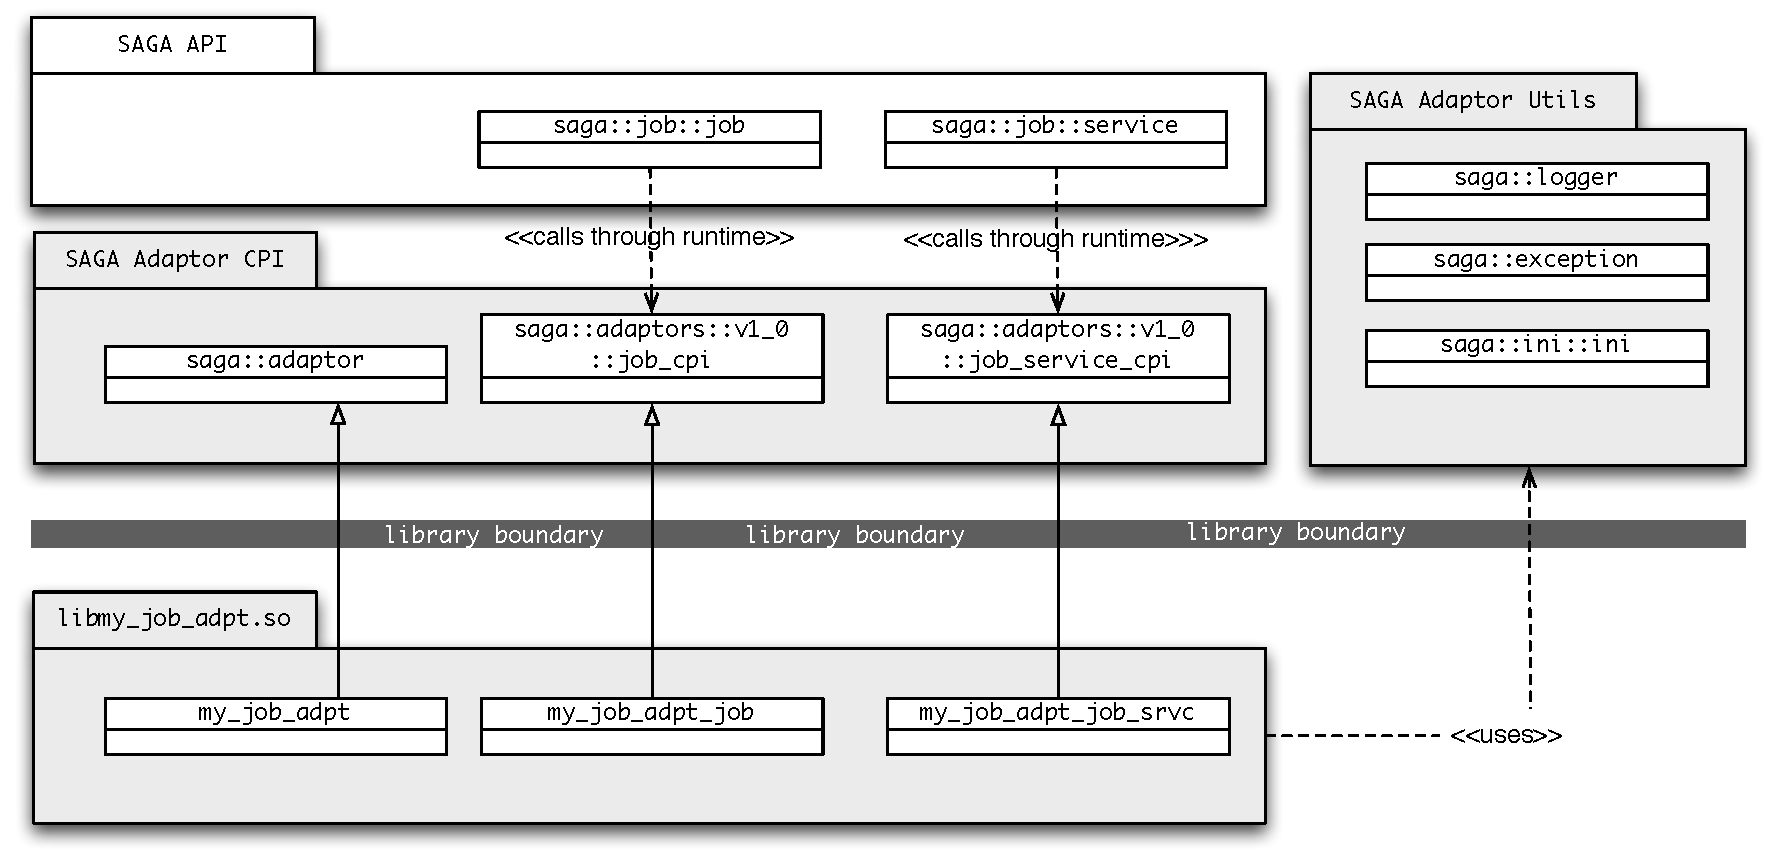
\includegraphics[scale=0.5]{figures/cpi-detail}
 \end{center}
 \caption{TODO}
\label{fig:cpi-detail}
\end{figure}

 
 \onote{Mention instancedata, adaptordata, ...}
 
 \subsubsection{Adaptors for Task Execution and Management}
 The various job adaptors obviously \textbf{O.W}
 
 \subsubsection{Adaptors for Data Access and Management}
 In the wake of a new important class of distributed applications that focus on 
 complex - often sensor-driven - data-intensive scientific workflows, data 
 management and access capabilities are becoming incresingly important for 
 application developers. Although SAGA does not provide a high-level abstraction
 for \textit{data} per se, it provides several functional packages that allow 
 and simplify low-level data access. These package APIs can easily be used to 
 develop a data abstraction framework on-top-of SAGA. The following list gives an
 overview of functional packages and adaptors that support data access and 
 management:
 
 \begin{itemize}

\item \textbf{File Package} - \onote{Short Description}

\begin{itemize}
\item Globus GridFTP File Adaptor
\item HDFS File Adaptor
\item Local File Adaptor
\item SSH File Adaptor

\end{itemize}

\item \textbf{Advert Package} - \onote{Short Description}

\begin{itemize}
\item PostgreSQL Advert Adaptor
\item SQLite3 Advert Adaptor
\end{itemize}

\item \textbf{Replica Package} - \onote{Short Description}

\begin{itemize}
\item PostgreSQL/SQLite3 Replica Adaptor
\item Globus RLS Replica Adaptor
\end{itemize}

\item \textbf{Stream Package}

\begin{itemize}
\item TCP Socket Stream Adaptor
\end{itemize}

\end{itemize}
 
 %This can (should)  include data as well as advert and replica adaptors \textbf{O.W}


 \subsubsection{Adaptors Bindings}
 Whatever else is worth mentioning: streams, sd, ... \textbf{O.W}


 \subsubsection{Package and Delivery} (AM)

 \subsection{Python Language Bindings}
 \textbf{H.K., O.W}
 
 
 \subsection{Performance Aspects}
 T.B.D. (Look at old Globus adaptor benchmarks, etc..) \textbf{O.W}

 \subsection{Development Process}
 software architecture and development process and how it is designed to encourage and facilitate community contribution \textbf{O.W}

\subsection{Error Handling}

\jhanote{Ideally this subsection will describe how SAGA does or does
  not address many/all elements of error handling in a distributed
  environment}

\subsection{Regression Testing}
\jhanote{We need a subsection on regression testing. Can't have a
  paper on production grade software without some description of
  testing process, and possibly also release/packaging (though far
  less important)}

